%Beschreibung der Implementierung der Kommunikation mit & Auswertung der Werte von dem Gyro

\subsection{Hardware}
Für die Ermittlung der Position des Würfels wurde ein digital Beschleunigungsmesser verwendet. Für ein Projekt standen zwei Beschleunigungsmesser zur Verfügung: BNO055 von Adafruit und ADXL345 von Analog Devices. Zwar ein Beschleunigungsmesser von Adafruit mächtiger ist und mehr Messungen erlaubt, das Projekt wurde am Ende unter der Verwendung des Beschleunigungsmessers ADXL345 geschrieben. Nach mehreren Versuchen, mit Adafruit zu arbeiten, wurde es festgestellt, dass Beschleunigungsmesser nicht arbeitsfähig ist. In alle Registern des Bausteins anstatt der vorprogrammierte Daten liegt nur die Zahl "0xe5", was laut der Hersteller zeigt, dass Registern irgendwie geleert wurden.\\

Für die Verwendung des ADXL345 sollte man in Programm nur die Adressen ändern und richtig alle Pins belegen. Die ALT ADDRESS wurde auf 1 gesetzt und die 7-Bit-I2C-Adresse für das Gerät wurde somit als "0x1D" festgelegt. In Programm wurde direkt dir entsprechende 8-Bir-I2C-Adresse "0x3A" verwendet und die notwendige Änderung der Adresse in "0x3B" aus "0x3A" wurde gerade in I2C Routine erledigt. So kann man unterscheiden, ob es Lesen oder Schreiben Operation durchführen sollen werden. \\

Es gibt keine internen Pull-Up- oder Pull-Down-Widerstände für nicht verwendete Pins. Daher gibt es keinen bekannten Status oder Standardstatus für den CS- oder ALT ADDRESS-Pin, wenn er potentialfrei bleibt oder nicht verbunden ist. Es ist erforderlich, dass der CS-Pin an VDD  angeschlossen ist und dass der ALT ADDRESS-Pin bei Verwendung von I2C entweder an VDD oder GND angeschlossen ist (wir haben an VDD angeschlossen).\\

Die gemessene Daten werden aus die Register 0x32 bis Register 0x37 gelesen. Diese sechs Bytes (Register 0x32 bis Register 0x37) sind jeweils acht Bits und enthalten die Ausgangsdaten für jede Achse. Register 0x32 und Register 0x33 enthalten die Ausgangsdaten für die X-Achse, Register 0x34 und Register 0x35 die Ausgangsdaten für die Y-Achse und Register 0x36 und Register 0x37 die Ausgangsdaten für die Z-Achse. \\

Die Ausgangsdaten sind zwei Komplemente, mit DATAx0 als niedrigstwertigem Byte und DATAx1 als höchstwertigem Byte, wobei x X, Y oder Z darstellt. Um die Daten richtig zu lesen, wurde es ein Mehrbyte-Lesen von 2 Register durchgeführt und die Daten aus zwei Lesevorgängen nach dem Lesen als 16-Bit Ausgangsdaten dargestellt. 

\begin{lstlisting}
uint16_t i2c16bit = 0x00;
ReadLenght = 2;
GlobalI2CAddr = addr;
I2CMasterBuffer[0] = regs[0];
I2CMasterBuffer[1] = regs[1];
...
// merge the data from two registers
i2c16bit = i2c16bit | I2CReadBuffer[1]; // [REG0, REG1]: REG1 as MSB
i2c16bit = i2c16bit << 8;

i2c16bit = i2c16bit | I2CReadBuffer[0]; // [REG0, REG1]: REG0 as LSB

\end{lstlisting}

\subsection{I2C: Grundlagen und Realisierung auf dem Keil Board}
Für unseres Projekt haben wir I2C Block auf dem Keil Board in Master-Modus programmiert. Mit Master-Sendermodus werden Daten vom Master (Keil Board) zum Slave (Beschleunigungsmesser) übertragen. So erlaubt uns den Beschleunigungsmesser zu initialisieren. \\

Im Master-Empfängermodus werden Daten von einem Slave-Sender empfangen. Nach der Initialisierung des Beschleunigungsmessers wird es immer weiter in diesem Modus gearbeitet, da wir nur ständig die ermittelte Position ablesen wollen. \\

Für unseres Projekt haben wir I2C1 Block gewählt. Mithilfe von Schaltbild haben wir festgestellt, welche Pins stehen uns zu Verfügung und sind mit anderen Peripheriefunktionen, die während unseres Projekt notwendig sein könnten, nicht belegt. 

\begin{figure}[!hb]
	\centering
	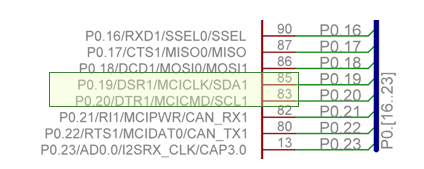
\includegraphics[width=0.6\linewidth]{pins_gyro.jpg}
	\caption[I2C1 Pin Belegung]{2C1 Pin Belegung}
	\label{fig:i2cpins}
\end{figure}

Das PCONP-Register ermöglicht das Deaktivieren ausgewählter Peripheriefunktionen, um Energie zu sparen. Wenn ein Peripheriesteuerbit 1 ist, ist dieses Peripheriegerät aktiviert. Wenn ein Peripherie-Bit 0 ist, wird die Uhr des Peripheriegeräts deaktiviert, um Energie zu sparen. Dem I2C1 entspricht das Bit 19 in PCONP-Register. Um I2C1 zu aktivieren, muss man den Wert $2^{19}$ ins Register schreiben, was in Hexadezimal Format $0x00080000$ entspricht. Mit der Verwendung von logischen Operator $OR$ wird die I2C1 aktiviert und die andere Peripheriefunktionen unverändert geblieben.
\begin{lstlisting}
PCONP |= 0x00080000;
\end{lstlisting}
Die nächste Schritte erlauben es, die Interrupt zu aktivieren. Da dem I2C1 das Bit 19 entspricht, wird es immer mit 19 Bit in jedem Register gearbeitet. Vector Address Registers 0-31 (VICVectAddr0-31 sind schreibgeschützte Register. Diese Register enthalten die Adressen der Interrupt-Service-Routinen (ISRs) für die 32 vektorisierten IRQ-Slots.
\begin{lstlisting}
VICVectCntl19 = 0x0000001;   // select a priority slot for interrupt
VICVectAddr19 = (unsigned)i2c_irq; //pass the address of the IRQ
VICIntEnable |= 0x00080000; // enable interrupt
PINSEL1 |= 0x000003C0; //Switch GPIO to I2C pins
\end{lstlisting}

Als nächstes wird ein Auswahl der geeigneten I2C-Datenrate und des Arbeitszyklus durchgeführt. Man muss Werte für die Register I2SCLH und I2SCLL einstellen, um die entsprechende Datenrate und den entsprechenden Arbeitszyklus auszuwählen. I2SCLH definiert die Anzahl der PCLK-Zyklen für die SCL-Hochzeit, I2SCLL definiert die Anzahl der PCLK-Zyklen für die SCL-Niedrigzeit. Dafür wird die folgende Formel benutzt:

\begin{equation}
I^2C_{bitfrequency} =  \frac{F_{PCLK}}{I2SCLH + I2SCLL }
\end{equation}\\

Da es mit der Frequenz von 400KHz gearbeitet wird, wird ins PCONP-Register die entsprechenden Werte geschrieben:
\begin{lstlisting}
I21SCLH = 0xF;
I21SCLL  = 0xF;
\end{lstlisting}

Steuerregister I2CONSET und I2CONCLR enthalten Bits, die zur Steuerung der folgenden I2C-Blockfunktionen verwendet werden: Start und Neustart einer seriellen Übertragung, Beenden einer seriellen Übertragung, Bitrate, Adresserkennung und Bestätigung. Der Inhalt des I2C-Steuerregisters kann als I2CONSET gelesen werden. Beim Schreiben auf I2CONSET werden Bits im I2C-Steuerregister gesetzt, die denen im geschriebenen Wert entsprechen. Umgekehrt löscht das Schreiben in I2CONCLR Bits im I2C-Steuerregister, die denen im geschriebenen Wert entsprechen. Während die Initialisierung wird folgendes in die I2CONSET und I2CONCLR geschrieben: \\

\begin{lstlisting}
I21CONCLR = 0x000000FF; // Clear all I2C settings
I21CONSET = 0x00000040; // Enable the I2C interface
\end{lstlisting}

Schieberegister I2DAT enthält ein Byte der zu übertragenden seriellen Daten oder ein gerade empfangenes Byte. Daten in I2DAT werden immer von rechts nach links verschoben. Das erste zu sendende Bit ist das MSB (Bit 7), und nachdem ein Byte empfangen wurde, befindet sich das erste Bit der empfangenen Daten im MSB von I2DAT. \\

Der Master-Sendermodus kann jetzt durch Setzen des STA-Bits aufgerufen werden. Die I2C-Logik testet nun den I2C-Bus und generiert eine Startbedingung, sobald der Bus frei wird. Wenn eine START-Bedingung übertragen wird, wird das serielle Interrupt-Flag (SI) gesetzt und der Statuscode im Statusregister (I2STAT) wird 0x08 sein. Dieser Statuscode wird von der Interrupt-Service-Routine verwendet, um die entsprechende Status-Service-Routine einzugeben, die I2DAT mit der Slave-Adresse und dem Datenrichtungsbit (SLA + W) lädt.\\

Im Master-Empfängermodus werden einige Datenbytes von einem Slave-Sender empfangen. Die Übertragung wird wie im Mastersender-Modus initialisiert. Wenn die Startbedingung übertragen wurde, muss die Interrupt-Service-Routine I2DAT mit der 7-Bit-Slave-Adresse und dem Datenrichtungsbit (SLA + R) laden. Wenn die Slaveadresse und das Datenrichtungsbit gesendet und ein Bestätigungsbit empfangen wurde, wird das serielle Interrupt-Flag (SI) erneut gesetzt und eine Nummer festgelegt Statuscodes in I2STAT sind möglich. 


\subsection{Software}

%

\begin{lstlisting}
unsigned int ADXLI2CAdresss = 0x3A;

\end{lstlisting}


\subsection{Probleme und Lösungen}